\documentclass[conference]{IEEEtran}

\usepackage{amsmath,amssymb}
\usepackage{booktabs}
\usepackage{graphicx}
\usepackage{hyperref}
\usepackage{cleveref}
\usepackage{algorithm}
\usepackage{algpseudocode}
\usepackage{xcolor}
\usepackage{enumitem}
\usepackage{caption}
\usepackage{subcaption}
\usepackage{listings}
\usepackage{microtype}
\usepackage{multirow}
\usepackage{tabularx}
\usepackage{tikz}
\usepackage{pgfplots}
\pgfplotsset{compat=1.18}
\usetikzlibrary{arrows.meta,positioning,calc}

\hypersetup{
  colorlinks=true,
  linkcolor=blue!70!black,
  citecolor=green!50!black,
  urlcolor=blue!60!black,
}

\lstset{
  language=Python,
  basicstyle=\ttfamily\scriptsize,
  keywordstyle=\color{blue!70!black}\bfseries,
  commentstyle=\color{green!50!black}\itshape,
  stringstyle=\color{red!60!black},
  breaklines=true,
  frame=single,
  framesep=2pt,
  rulecolor=\color{gray!40},
}

\newcommand{\ncsim}{\texttt{ncsim}}
\newcommand{\dBm}{\,\text{dBm}}
\newcommand{\dB}{\,\text{dB}}
\newcommand{\mW}{\,\text{mW}}
\newcommand{\MHz}{\,\text{MHz}}
\newcommand{\GHz}{\,\text{GHz}}
\newcommand{\Mbps}{\,\text{Mbps}}
\newcommand{\MBps}{\,\text{MB/s}}

\title{\ncsim{}: A Lightweight Discrete-Event Simulator\\for Networked Computing with 802.11 WiFi Models}
\author{
\IEEEauthorblockN{Bhaskar Krishnamachari\IEEEauthorrefmark{1},
Maya Gutierrez\IEEEauthorrefmark{1}, and
Jared Coleman\IEEEauthorrefmark{1}\IEEEauthorrefmark{2}}
\IEEEauthorblockA{\IEEEauthorrefmark{1}University of Southern California\\
bkrishna@usc.edu, mayaguti@usc.edu}
\IEEEauthorblockA{\IEEEauthorrefmark{2}Loyola Marymount University\\
jared.coleman@lmu.edu}
}

\begin{document}
\maketitle

%% ============================================================
\begin{abstract}
We present \ncsim{}, a deterministic discrete-event simulator for evaluating
task scheduling algorithms on heterogeneous networked computing systems.
\ncsim{} models directed acyclic graph (DAG) workflows, multi-hop routing
with bandwidth sharing, and IEEE~802.11 WiFi links with a
physically-grounded CSMA/CA interference model based on Bianchi's analysis,
including contention and hidden terminal SINR degradation.
The simulator supports pluggable scheduling
algorithms (including HEFT and CPOP via the SAGA library) and three routing
strategies.
Implemented in approximately 5,500 lines of Python with YAML-driven scenario
specification, \ncsim{} fills a gap between heavyweight network simulators
like ns-3 and task-centric simulators like SimGrid, enabling rapid
exploration of the interplay between compute placement and network transport
in edge and fog computing deployments.  We validate the WiFi model against
analytical predictions across nine experiments, achieving exact match within
1\% tolerance in all cases.
\end{abstract}

%% ============================================================
\section{Introduction}
\label{sec:intro}

Edge and fog computing architectures distribute computation across
heterogeneous nodes connected by networks of varying capacity and
reliability~\cite{shi2016edge}.  Effective task scheduling in these
environments requires co-optimizing compute placement and network transport:
a task placement that minimizes computation time may incur excessive data
transfer costs, while a network-aware placement may underutilize fast
processors.

Existing simulation tools address parts of this problem.  Network simulators
such as ns-3~\cite{ns3} and OMNeT++~\cite{omnetpp} provide detailed protocol
stacks but are heavyweight, complex to configure, and lack native support for
DAG-based task scheduling.  Conversely, task scheduling simulators such as
SimGrid~\cite{simgrid}, WRENCH~\cite{wrench}, and CloudSim~\cite{cloudsim}
model workflows and compute resources but typically abstract the network as
point-to-point links with fixed bandwidths, omitting wireless contention,
interference, and multi-hop effects.

We present \ncsim{}, a lightweight discrete-event simulator that bridges this
gap.  \ncsim{} combines DAG workflow scheduling with physically-grounded
802.11 WiFi models in a single, easy-to-use Python package.  Our
contributions are:

\begin{itemize}[itemsep=2pt,leftmargin=*]
\item A modular simulation architecture with abstract base classes for
  schedulers, routing models, interference models, link models, and queue
  models, enabling pluggable experimentation.
\item An 802.11 WiFi model incorporating log-distance path loss, MCS rate
  adaptation (802.11n/ac/ax), conflict graph construction, CSMA/CA contention
  via Bianchi's analysis, and hidden terminal SINR degradation.
\item Multi-hop routing with dynamic bandwidth sharing and three routing
  strategies (direct, widest-path, shortest-path).
\item Experimental validation demonstrating exact match between simulated and
  analytically predicted behavior across nine verification experiments.
\item An open-source implementation in ${\sim}5{,}500$ lines of Python with
  YAML-driven scenarios, JSONL trace output, and a React/D3 visualization
  frontend.
\end{itemize}

%% ============================================================
\section{Related Work}
\label{sec:related}

\textbf{Network simulators.}
ns-3~\cite{ns3} is a widely-used discrete-event network simulator with
detailed WiFi, LTE, and TCP/IP models.  OMNeT++~\cite{omnetpp} with the INET
framework provides similar capabilities in a component-based architecture.
Both excel at protocol-level analysis but require substantial expertise to
configure, and neither provides native DAG scheduling or workflow management.
Researchers studying task placement in wireless networks must integrate
external schedulers manually.

\textbf{Task scheduling simulators.}
SimGrid~\cite{simgrid} models distributed computing platforms with
analytical network models and supports DAG workflows.  WRENCH~\cite{wrench}
builds on SimGrid to provide workflow management system simulation.
CloudSim~\cite{cloudsim} targets cloud computing with VM-level abstractions.
These tools model networks as links with fixed or analytically-derived
bandwidths, without wireless contention, hidden terminal effects, or
carrier-sense-based spatial reuse.

\textbf{Edge/fog-specific simulators.}
iFogSim~\cite{ifogsim} extends CloudSim for fog computing topologies.
EdgeCloudSim~\cite{edgecloudsim} adds mobility and WLAN models.  These
provide domain-specific features but use simplified wireless models
(typically constant bandwidth with optional capacity degradation) that do not
capture the distance-dependent rates, CSMA contention, or hidden terminal
interference that characterize real 802.11 deployments.

\textbf{Positioning of \ncsim{}.}
\ncsim{} occupies a unique position: it combines DAG-aware task scheduling
with 802.11 physical-layer fidelity (SNR-based rate adaptation, Bianchi MAC
efficiency, SINR-based hidden terminal modeling) in a lightweight Python
package.  Unlike ns-3, it does not simulate packet-level protocol stacks;
unlike SimGrid, it does not abstract away wireless interference.  This makes
it well-suited for rapid exploration of scheduling algorithms in wireless
edge computing scenarios where both compute placement and wireless network
effects matter.

%% ============================================================
\section{Architecture}
\label{sec:arch}

\ncsim{} follows a layered architecture organized around a discrete-event
simulation (DES) engine.  \Cref{fig:architecture} illustrates the data flow.

\begin{figure}[t]
\centering
\fbox{\parbox{0.93\columnwidth}{\small
\textbf{Input:} Scenario YAML $\rightarrow$ Scenario Loader\\[3pt]
$\downarrow$\\[2pt]
\textbf{Core:} Network + DAGs + Config\\[2pt]
$\downarrow$\\[2pt]
\textbf{Simulation Engine}\\
\quad Event Queue (min-heap, 6 event types)\\
\quad Execution Engine (state machine)\\
\quad$\hookleftarrow$ Scheduler (HEFT, CPOP, RoundRobin, Manual)\\
\quad$\hookleftarrow$ Routing Model (Direct, Widest, Shortest)\\
\quad$\hookleftarrow$ Interference Model (None, CSMA Bianchi)\\[2pt]
$\downarrow$\\[2pt]
\textbf{Output:} JSONL Trace + Metrics JSON
}}
\caption{High-level architecture of \ncsim{}.}
\label{fig:architecture}
\end{figure}

\subsection{Design Goals}

\textbf{Determinism.}  Given the same scenario and random seed, \ncsim{}
produces identical results across runs.  Floating-point times are rounded to
microsecond precision to prevent accumulation errors.

\textbf{Modularity.}  Six abstract base classes (ABCs) define clean extension
points: \texttt{Scheduler}, \texttt{RoutingModel}, \texttt{InterferenceModel},
\texttt{LinkModel}, \texttt{QueueModel}, and \texttt{DAGSource}.  New
strategies can be added without modifying the core engine.

\textbf{Simplicity.}  Scenarios are specified in YAML.  The entire simulator
is implemented in Python with minimal dependencies (only the optional SAGA
library for HEFT/CPOP).

\textbf{Physical grounding.}  Wireless link bandwidths are derived from RF
parameters (transmit power, frequency, path loss exponent) rather than
specified as arbitrary constants.

\subsection{Design Trade-offs}

\ncsim{} intentionally omits several features to maintain its lightweight,
fast character while retaining the key phenomena---contention, hidden
terminals, MCS adaptation---that affect scheduling decisions:

\begin{itemize}[itemsep=1pt,leftmargin=*]
\item \textbf{No packet-level simulation.}  There is no TCP/IP stack or
  per-packet event processing; transfers are modeled as bulk flows with
  analytically-derived rates.
\item \textbf{No physical-layer channel dynamics.}  Fading, OFDM subcarrier
  allocation, and time-varying channel states are not modeled; path loss is
  static and deterministic (with optional log-normal shadow fading).
\item \textbf{No mobility.}  The topology is static; node positions are fixed
  for the duration of a simulation run.
\item \textbf{Single-slot compute.}  Each node executes one task at a time
  (FIFO queuing); GPU-like multi-slot parallelism is left to future work.
\end{itemize}

\noindent These choices keep simulation runtimes on the order of seconds for
networks of up to 16 nodes and 20-task DAGs, enabling rapid parameter sweeps
that would be infeasible with packet-level simulators.

\subsection{Key Abstractions}

\Cref{tab:abstractions} summarizes the six pluggable abstractions in \ncsim{}.

\begin{table}[t]
\centering
\caption{Pluggable abstractions in \ncsim{}.}
\label{tab:abstractions}
\begin{tabular}{@{}lp{4.8cm}@{}}
\toprule
\textbf{ABC} & \textbf{Implementations} \\
\midrule
Scheduler & Manual, RoundRobin, HEFT, CPOP \\
RoutingModel & Direct, WidestPath, ShortestPath \\
InterferenceModel & None, CSMA Bianchi \\
LinkModel & Static (future: position-based, TDMA) \\
QueueModel & FIFO (future: priority, multi-slot) \\
DAGSource & Single, Multi \\
\bottomrule
\end{tabular}
\end{table}

%% ============================================================
\section{System Model}
\label{sec:model}

\subsection{Network Model}

A network consists of \emph{nodes} and directed \emph{links}.  Each node $v$
has a compute capacity $C_v$ (compute units per second) and an optional 2D
position $(x_v, y_v)$ used for RF calculations.  Each link $\ell$ from node
$u$ to node $v$ has a bandwidth $B_\ell$ (MB/s) and latency $L_\ell$
(seconds).  Topologies are specified in YAML and can be arbitrary directed
graphs.

\subsection{Compute Model}

A task $t$ has a compute cost $w_t$ (in compute units).  The execution time
on node $v$ is $w_t / C_v$.  Each node processes one task at a time using
FIFO queuing.  Tasks follow a five-state lifecycle: \textsc{Pending}
$\rightarrow$ \textsc{Ready} $\rightarrow$ \textsc{Queued} $\rightarrow$
\textsc{Running} $\rightarrow$ \textsc{Completed}.

\subsection{DAG Workflow Model}

Workflows are modeled as directed acyclic graphs (DAGs) where nodes represent
tasks and edges represent data dependencies.  Each edge $e = (t_i, t_j)$
carries a data payload of size $d_e$ (in MB) that must be transferred from
the node executing $t_i$ to the node executing $t_j$ before $t_j$ can begin.
If $t_i$ and $t_j$ are placed on the same node, the transfer is
instantaneous (zero cost).  DAGs are injected at specified simulation times.

\subsection{Scheduling Framework}

The scheduler receives a \texttt{NetworkSnapshot}---an immutable view of
node capacities, link bandwidths, queue depths, and active transfers---and
returns a \texttt{PlacementPlan} mapping each task to a node.  \ncsim{}
includes four schedulers:

\begin{itemize}[itemsep=1pt,leftmargin=*]
\item \textbf{Manual:} Uses \texttt{pinned\_to} annotations from the YAML.
\item \textbf{RoundRobin:} Cycles through nodes, respecting pin constraints.
\item \textbf{HEFT/CPOP:} Adapted from the SAGA scheduling library via an
  adapter that constructs a fully-connected virtual network with actual
  bandwidths for connected pairs and near-zero bandwidth for unreachable
  pairs, causing the scheduler to naturally avoid infeasible placements.
\end{itemize}

\subsection{Routing and Bandwidth Sharing}

Three routing models determine the path for data transfers:

\begin{itemize}[itemsep=1pt,leftmargin=*]
\item \textbf{Direct:} Only allows transfers over explicit single-hop links.
\item \textbf{WidestPath:} Modified Dijkstra maximizing bottleneck bandwidth.
\item \textbf{ShortestPath:} Standard Dijkstra minimizing total latency.
\end{itemize}

Multi-hop transfers use store-and-forward semantics: the effective bandwidth
is the minimum (bottleneck) across all links in the path, and latency is the
sum.  When multiple transfers share a link, each receives a fair share:
\begin{equation}
B_\text{per-flow}(\ell) = \frac{B_\ell \cdot f(\ell)}{N_\ell}
\label{eq:fair_share}
\end{equation}
where $f(\ell)$ is the interference factor and $N_\ell$ is the number of
concurrent flows on link $\ell$.  When a transfer starts or completes, all
affected transfers are recalculated and their completion events rescheduled.

\subsection{WiFi / 802.11 Model}
\label{sec:wifi}

The WiFi model replaces static link bandwidths with rates derived from RF
parameters, and replaces simple interference factors with physically-grounded
contention and hidden terminal models.

\subsubsection{Physical Layer}

The received power at distance $d$ uses log-distance path loss:
\begin{align}
\text{PL}(d) &= \text{PL}(d_0) + 10\,n\,\log_{10}\!\left(\frac{d}{d_0}\right) \label{eq:pathloss} \\
P_\text{rx}(d) &= P_\text{tx} - \text{PL}(d) \label{eq:rxpower}
\end{align}
where $\text{PL}(d_0)$ is the Friis free-space loss at reference distance
$d_0 = 1$\,m, $n$ is the path loss exponent, and $P_\text{tx}$ is the
transmit power.  The signal-to-noise ratio is $\text{SNR} = P_\text{rx} - N_0$
(in dB), where $N_0$ is the noise floor.

The PHY data rate is selected from 802.11n/ac/ax MCS tables:
\begin{equation}
R_\ell = \max\{r_k : \text{SNR}_\ell \geq \text{SNR}_{\min,k}\}
\label{eq:mcs}
\end{equation}
For example, at 5\,GHz with $n = 3$, a 30\,m link achieves SNR $= 24.3$\,dB,
selecting MCS~5 (64-QAM~2/3) at 68.8\,Mbps $= 8.6$\,MB/s under 802.11ax.

\subsubsection{Carrier Sensing and Conflict Graph}

The carrier sensing range $d_\text{CS}$ is the maximum distance at which a
transmission triggers the clear channel assessment (CCA) mechanism:
\begin{equation}
d_\text{CS} = d_0 \cdot 10^{\,\frac{P_\text{tx} - \theta_\text{CCA} - \text{PL}(d_0)}{10\,n}}
\label{eq:csrange}
\end{equation}

The conflict graph $G_C = (L, E_C)$ is defined over links.  Without RTS/CTS,
two links conflict if either transmitter can sense any node of the other
link.  With RTS/CTS, any node of one link sensing any node of the other
creates a conflict.

\subsubsection{CSMA Bianchi Model (\texttt{csma\_bianchi})}
\label{sec:bianchi}

The dynamic model separates two interference mechanisms.  Let $\mathcal{A}$
be the set of currently active links, $\mathcal{C}_\ell = \mathcal{A} \cap
\mathcal{N}(\ell)$ the active contending neighbors, and $\mathcal{H}_\ell =
(\mathcal{A} \setminus \mathcal{N}(\ell)) \setminus \{\ell\}$ the active
hidden terminals.

\paragraph{Contention factor.}
The number of contending stations is $n = 1 + |\mathcal{C}_\ell|$.  Using
Bianchi's saturation throughput analysis~\cite{bianchi2000}, the MAC
efficiency $\eta(n)$ is computed from the coupled equations for transmission
probability $\tau$ and collision probability $p$:
\begin{align}
\tau &= \frac{2(1 - 2p)}{(1 - 2p)(W_{\min} + 1) + p\,W_{\min}(1 - (2p)^m)} \label{eq:tau} \\
p &= 1 - (1 - \tau)^{n-1} \label{eq:p}
\end{align}
with $W_{\min} = 16$ and $m = 6$.  The efficiency is:
\begin{equation}
\eta(n) = \frac{P_\text{success} \cdot T_\text{success}}{\mathbb{E}[T_\text{slot}]}
\label{eq:eta}
\end{equation}
Each contending station receives a share $\eta(n)/n$ of the channel.

\paragraph{SINR factor.}
Hidden terminals cause interference at the receiver.  The SINR is:
\begin{equation}
\text{SINR}_\ell = 10\log_{10}\!\left(\frac{P_\text{rx}^{(\text{lin})}}{N_0^{(\text{lin})} + \sum_{j \in \mathcal{H}_\ell} P_j^{(\text{lin})}}\right)
\label{eq:sinr}
\end{equation}
The degraded rate $R_\text{SINR}$ is looked up from the MCS table, giving
$f_\text{SINR} = R_\text{SINR}/R_\ell$.

\paragraph{Combined factor.}
\begin{equation}
\boxed{f(\ell) = \frac{R_\text{SINR}(\ell)}{R_\ell} \cdot \frac{\eta(n)}{n}}
\label{eq:combined}
\end{equation}
clamped to $[0.01, 1.0]$.  When transfers start or complete, all active
conflict graph neighbors are recalculated and their completion events
rescheduled.

%% ============================================================
\section{Simulation Engine}
\label{sec:engine}

\ncsim{} uses an event-driven DES with a min-heap priority queue.  Six event
types are processed in priority order at each simulation time:

\begin{enumerate}[itemsep=1pt,leftmargin=*]
\item \textsc{DagInject} --- Invokes scheduler, initializes task states
\item \textsc{TaskComplete} --- Frees node, triggers output transfers
\item \textsc{TransferComplete} --- Delivers data, checks readiness
\item \textsc{TaskReady} --- Starts task or enqueues if node busy
\item \textsc{TaskStart} --- Begins execution, schedules completion
\item \textsc{TransferStart} --- Acquires link bandwidth, schedules completion
\end{enumerate}

This ordering ensures causal correctness: completions are processed before
starts at the same simulation time, and task completions before transfer
completions so that freed nodes can accept new work immediately.

Events are cancellable via lazy deletion, used when bandwidth recalculation
invalidates a previously-scheduled completion time.  All times are rounded to
microsecond precision ($10^{-6}$\,s) to ensure deterministic behavior across
platforms.

%% ============================================================
\section{Experimental Evaluation}
\label{sec:eval}

We evaluate \ncsim{} through three sets of experiments: WiFi model
validation against analytical predictions, routing strategy comparison, and
interference impact analysis.

\subsection{WiFi Model Validation}
\label{sec:validation}

We validate the \texttt{csma\_bianchi} model against analytical predictions
computed directly from the WiFi RF equations, using a 1\% match tolerance.
Nine experiments were conducted; all achieve exact match.

\subsubsection{Experiment 1: Link Length vs.\ Data Rate}

A single link between two nodes at varying distances from 1\,m to 140\,m.
\Cref{tab:exp1} shows selected results.  The simulated rate matches the
analytically predicted MCS-selected rate at every distance.  At 140\,m the
SNR (4.19\,dB) falls below MCS~0 (5\,dB threshold), correctly yielding zero
rate.  \Cref{fig:exp1} plots the characteristic staircase pattern: rate
is constant within each MCS band and drops discretely at each SNR threshold.

\begin{table}[t]
\centering
\caption{Experiment 1: Link length vs.\ data rate (802.11ax, 5\,GHz).}
\label{tab:exp1}
\begin{tabular}{@{}rrrrr@{}}
\toprule
\textbf{Dist(m)} & \textbf{SNR(dB)} & \textbf{MCS} & \textbf{Pred(MB/s)} & \textbf{Sim(MB/s)} \\
\midrule
1   & 68.58 & 11  & 17.925 & 17.925 \\
12  & 36.20 & 9   & 14.338 & 14.338 \\
30  & 24.27 & 5   & 8.600  & 8.600  \\
50  & 17.61 & 3   & 4.300  & 4.300  \\
75  & 12.33 & 2   & 3.225  & 3.225  \\
105 & 7.94  & 0   & 1.075  & 1.075  \\
140 & 4.19  & n/a & 0.000  & 0.000  \\
\bottomrule
\end{tabular}
\end{table}

\begin{figure}[t]
\centering
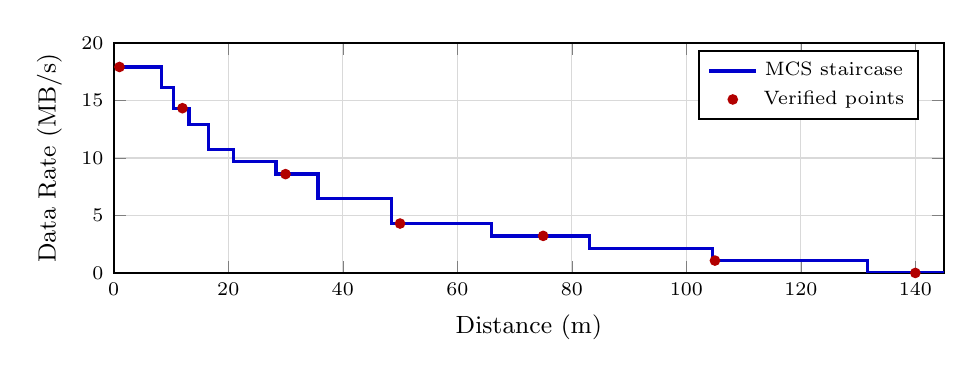
\begin{tikzpicture}
\begin{axis}[
  width=\columnwidth,
  height=4.5cm,
  xlabel={Distance (m)},
  ylabel={Data Rate (MB/s)},
  xmin=0, xmax=145,
  ymin=0, ymax=20,
  grid=major,
  grid style={gray!30},
  thick,
  legend pos=north east,
  legend style={font=\scriptsize},
  every axis label/.style={font=\small},
  tick label style={font=\scriptsize},
]
\addplot[blue!80!black, very thick]
  coordinates {
    (1, 17.925) (8.30, 17.925)
    (8.30, 16.125) (10.46, 16.125)
    (10.46, 14.338) (13.16, 14.338)
    (13.16, 12.900) (16.57, 12.900)
    (16.57, 10.750) (20.86, 10.750)
    (20.86, 9.675) (28.36, 9.675)
    (28.36, 8.600) (35.70, 8.600)
    (35.70, 6.450) (48.53, 6.450)
    (48.53, 4.300) (65.97, 4.300)
    (65.97, 3.225) (83.05, 3.225)
    (83.05, 2.150) (104.55, 2.150)
    (104.55, 1.075) (131.62, 1.075)
    (131.62, 0) (145, 0)
  };
\addplot[only marks, mark=*, mark size=1.5pt, red!70!black]
  coordinates {
    (1, 17.925) (12, 14.338) (30, 8.600) (50, 4.300)
    (75, 3.225) (105, 1.075) (140, 0)
  };
\legend{MCS staircase, Verified points}
\end{axis}
\end{tikzpicture}
\caption{Experiment 1: PHY data rate vs.\ link distance showing discrete MCS
  transitions (802.11ax, 5\,GHz, $n{=}3$).  Red dots mark experimentally
  verified data points from \Cref{tab:exp1}.}
\label{fig:exp1}
\end{figure}

\subsubsection{Experiment 2: Parallel Link Separation}

Two parallel 30\,m links separated vertically by distances from 5\,m to
200\,m.  \Cref{fig:exp2} illustrates the three interference regimes.
At separation $\leq 70$\,m, all node pairs are within the carrier
sensing range (71.2\,m), so the links \emph{contend} via Bianchi's model:
each gets $\eta(2)/2 \approx 0.44$ of the base rate 8.6\,MB/s $= 3.79$\,MB/s.
At separation $\geq 75$\,m, the links become hidden terminals, and SINR
degradation determines the effective rate.

Notably, the effective rate \emph{drops} at the CS range boundary---from
3.79\,MB/s (contention) to 3.23\,MB/s (hidden terminal at 75\,m)---before
recovering at larger separations.  This non-monotonic behavior is the
classic \emph{hidden terminal effect}: within sensing range, links coordinate
via CSMA/CA and time-share the channel fairly (each receiving 44\% of the
full 8.6\,MB/s); just outside sensing range, links transmit simultaneously
without coordination, and the resulting mutual interference degrades each
receiver's SINR enough to force a lower MCS rate (from MCS~5 to MCS~2).
The hidden terminal regime is thus \emph{worse} than fair contention sharing
at close range.  As separation increases further, interference power
diminishes: SINR recovers to MCS~3 (4.3\,MB/s) at 90\,m and MCS~4
(6.45\,MB/s) at 130\,m.  All 15 data points match predictions exactly.

\begin{figure}[t]
\centering
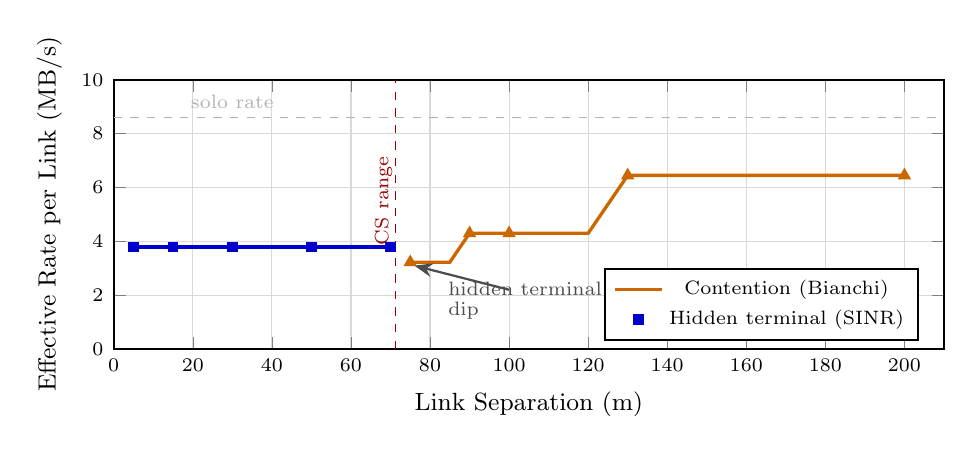
\begin{tikzpicture}
\begin{axis}[
  width=\columnwidth,
  height=5cm,
  xlabel={Link Separation (m)},
  ylabel={Effective Rate per Link (MB/s)},
  xmin=0, xmax=210,
  ymin=0, ymax=10,
  grid=major,
  grid style={gray!30},
  thick,
  every axis label/.style={font=\small},
  tick label style={font=\scriptsize},
  legend pos=south east,
  legend style={font=\scriptsize},
]
% Solo rate reference
\addplot[dashed, gray!60, thin] coordinates {(0, 8.600) (210, 8.600)};
\node[font=\scriptsize, gray!60] at (axis cs:30,9.2) {solo rate};

% CS range marker
\draw[dashed, red!60!black, thin] (axis cs:71.2,0) -- (axis cs:71.2,10);
\node[font=\scriptsize, red!60!black, rotate=90, anchor=south] at (axis cs:73,5.5) {CS range};

% Contention regime
\addplot[blue!80!black, very thick]
  coordinates {
    (5, 3.787) (10, 3.787) (15, 3.787) (20, 3.787) (25, 3.787)
    (30, 3.787) (35, 3.787) (40, 3.787) (45, 3.787) (50, 3.787)
    (55, 3.787) (60, 3.787) (65, 3.787) (70, 3.787)
  };

% Hidden terminal regime
\addplot[orange!80!black, very thick]
  coordinates {
    (75, 3.225) (80, 3.225) (85, 3.225)
    (90, 4.300) (95, 4.300) (100, 4.300) (110, 4.300) (120, 4.300)
    (130, 6.450) (140, 6.450) (150, 6.450) (175, 6.450) (200, 6.450)
  };

\addplot[only marks, mark=square*, mark size=1.5pt, blue!80!black]
  coordinates {
    (5, 3.787) (15, 3.787) (30, 3.787) (50, 3.787) (70, 3.787)
  };
\addplot[only marks, mark=triangle*, mark size=2pt, orange!80!black]
  coordinates {
    (75, 3.225) (90, 4.300) (100, 4.300) (130, 6.450) (200, 6.450)
  };

% Annotation: hidden terminal dip
\draw[-{Stealth}, thick, black!70] (axis cs:100,2.2) -- (axis cs:76,3.1);
\node[font=\scriptsize, anchor=west, align=left, black!70] at (axis cs:82,1.8)
  {hidden terminal\\[-1pt]dip};

\legend{, , Contention (Bianchi), Hidden terminal (SINR), , }
\end{axis}
\end{tikzpicture}
\caption{Experiment 2: Effective per-link rate vs.\ separation for two
  parallel 30\,m links.  Below the CS range (71.2\,m), links contend via
  Bianchi's model.  Above it, hidden terminal SINR degradation causes a
  non-monotonic \emph{dip}: the rate drops from 3.79 to 3.23\,MB/s at the
  boundary because uncoordinated simultaneous transmissions degrade SINR
  more than fair time-sharing reduces throughput.  Rate recovers as
  interference power falls with increasing distance.}
\label{fig:exp2}
\end{figure}

\subsubsection{Experiment 3: Two Transmitters to Same Receiver}

Two transmitter nodes at distance $d$ from a shared receiver, placed at 90
degrees.  The transmitter-to-transmitter distance is $d\sqrt{2}$.  At $d
\leq 70$\,m, both transmitters are within sensing range and contend via
Bianchi.  At $d = 75$\,m, they become hidden terminals with severe SINR
degradation (from 3.225 to 0.032\,MB/s).  All 18 points match.

\subsubsection{Additional Validation Experiments}

Six additional experiments validate: (4)~three-link topologies with mixed
contention and hidden terminal regimes, (5)~staggered transfer starts with
dynamic recalculation, (6)~per-link bandwidth sharing with multiple flows,
(7)~N-way Bianchi contention scaling from $n{=}2$ to $n{=}8$,
(8)~five-link hidden terminal cascades with different data sizes, and
(9)~combined bandwidth sharing with hidden terminal interference.  All pass.

\begin{table}[t]
\centering
\caption{Experiment 7: N-way Bianchi contention scaling (30\,m links at 5\,m
separation).  $\eta(n)$ is the Bianchi MAC efficiency.}
\label{tab:exp7}
\begin{tabular}{@{}rrrrrr@{}}
\toprule
$n$ & $\eta(n)$ & $\eta(n)/n$ & \textbf{Pred(MB/s)} & \textbf{Sim(MB/s)} \\
\midrule
2 & 0.881 & 0.440 & 3.787 & 3.787 \\
3 & 0.859 & 0.286 & 2.461 & 2.461 \\
4 & 0.837 & 0.209 & 1.799 & 1.799 \\
5 & 0.818 & 0.164 & 1.407 & 1.407 \\
6 & 0.802 & 0.134 & 1.149 & 1.149 \\
7 & 0.788 & 0.113 & 0.968 & 0.968 \\
8 & 0.726 & 0.091 & 0.780 & 0.780 \\
\bottomrule
\end{tabular}
\end{table}

\subsection{Routing Strategy Comparison}
\label{sec:routing_eval}

We compare widest-path and shortest-path routing under HEFT scheduling with
the \texttt{csma\_bianchi} interference model across grid mesh networks of
three sizes (2$\times$2, 3$\times$3, 4$\times$4) and three DAG complexities
(5, 10, and 20 tasks).  All links are wireless with 40\,m grid spacing.
Nodes have heterogeneous compute capacities (80--300 units/s).
\Cref{tab:routing} shows the results.

\Cref{fig:routing_diamond} illustrates \emph{why} routing strategy matters
using a diamond topology with asymmetric paths.  The widest-path algorithm
selects the high-bandwidth bottom path (200\,MB/s, 0.1\,s latency per hop),
achieving a makespan of 2.6\,s.  Shortest-path selects the low-latency top
path (20\,MB/s, 0.001\,s per hop), yielding 7.0\,s---a 2.7$\times$ slowdown
because the 100\,MB transfer dominates the total time.

\begin{figure}[t]
\centering
\begin{subfigure}[b]{\columnwidth}
\centering
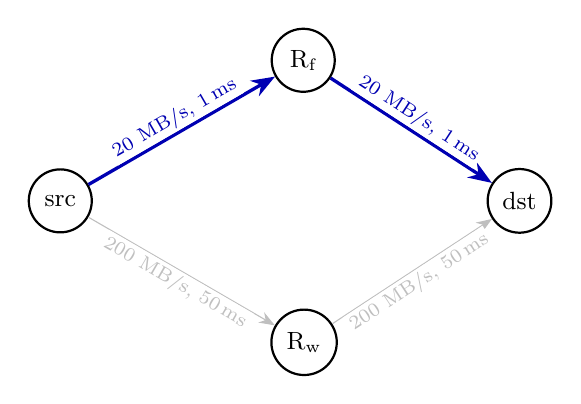
\begin{tikzpicture}[
  node distance=2cm and 2.8cm,
  nnode/.style={circle, draw, thick, minimum size=8mm, font=\small},
  sel/.style={-{Stealth[length=3mm]}, very thick, blue!70!black},
  dim/.style={-{Stealth[length=2mm]}, thin, gray!50},
  lbl/.style={font=\scriptsize, fill=white, inner sep=1pt},
]
  \node[nnode] (src) {src};
  \node[nnode, above right=1.2cm and 2.5cm of src] (fast) {R\textsubscript{f}};
  \node[nnode, below right=1.2cm and 2.5cm of src] (wide) {R\textsubscript{w}};
  \node[nnode, right=5cm of src] (dst) {dst};

  % Shortest path highlighted
  \draw[sel] (src) -- node[lbl, above, sloped] {20 MB/s, 1\,ms} (fast);
  \draw[sel] (fast) -- node[lbl, above, sloped] {20 MB/s, 1\,ms} (dst);

  % Wide path dimmed
  \draw[dim] (src) -- node[lbl, below, sloped] {200 MB/s, 50\,ms} (wide);
  \draw[dim] (wide) -- node[lbl, below, sloped] {200 MB/s, 50\,ms} (dst);
\end{tikzpicture}
\caption{Shortest-path routing selects the top path (lower latency).\\
  Makespan: $1.0 + (100/20 + 0.002) + 1.0 = 7.0$\,s.}
\end{subfigure}

\vspace{6pt}

\begin{subfigure}[b]{\columnwidth}
\centering
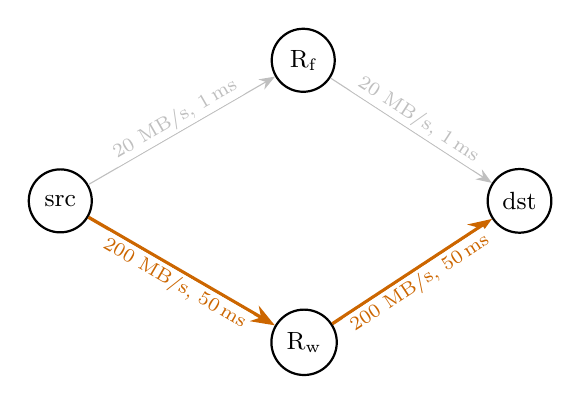
\begin{tikzpicture}[
  node distance=2cm and 2.8cm,
  nnode/.style={circle, draw, thick, minimum size=8mm, font=\small},
  sel/.style={-{Stealth[length=3mm]}, very thick, orange!80!black},
  dim/.style={-{Stealth[length=2mm]}, thin, gray!50},
  lbl/.style={font=\scriptsize, fill=white, inner sep=1pt},
]
  \node[nnode] (src) {src};
  \node[nnode, above right=1.2cm and 2.5cm of src] (fast) {R\textsubscript{f}};
  \node[nnode, below right=1.2cm and 2.5cm of src] (wide) {R\textsubscript{w}};
  \node[nnode, right=5cm of src] (dst) {dst};

  % Fast path dimmed
  \draw[dim] (src) -- node[lbl, above, sloped] {20 MB/s, 1\,ms} (fast);
  \draw[dim] (fast) -- node[lbl, above, sloped] {20 MB/s, 1\,ms} (dst);

  % Widest path highlighted
  \draw[sel] (src) -- node[lbl, below, sloped] {200 MB/s, 50\,ms} (wide);
  \draw[sel] (wide) -- node[lbl, below, sloped] {200 MB/s, 50\,ms} (dst);
\end{tikzpicture}
\caption{Widest-path routing selects the bottom path (higher bandwidth).\\
  Makespan: $1.0 + (100/200 + 0.1) + 1.0 = 2.6$\,s.}
\end{subfigure}
\caption{Routing strategy comparison on a diamond topology with a 100\,MB
  transfer.  When transfer size dominates, widest-path outperforms
  shortest-path by 2.7$\times$.}
\label{fig:routing_diamond}
\end{figure}

\begin{table}[t]
\centering
\caption{Routing comparison: makespan (seconds) for widest-path (W) vs.\
shortest-path (S) under HEFT with \texttt{csma\_bianchi}.}
\label{tab:routing}
\begin{tabular}{@{}llrrr@{}}
\toprule
\textbf{Network} & \textbf{DAG} & \textbf{W (s)} & \textbf{S (s)} & \textbf{Winner} \\
\midrule
\multirow{3}{*}{2$\times$2 (4 nodes)}
  & 5 tasks   & 11.43  & 11.43  & Tie \\
  & 10 tasks  & 20.52  & 26.03  & Widest \\
  & 20 tasks  & 51.65  & 38.94  & Shortest \\
\midrule
\multirow{3}{*}{3$\times$3 (9 nodes)}
  & 5 tasks   & 12.37  & 12.37  & Tie \\
  & 10 tasks  & 29.52  & 25.04  & Shortest \\
  & 20 tasks  & 46.01  & 40.82  & Shortest \\
\midrule
\multirow{3}{*}{4$\times$4 (16 nodes)}
  & 5 tasks   & 315.20 & 8.93   & Shortest \\
  & 10 tasks  & 967.21 & 434.13 & Shortest \\
  & 20 tasks  & 1472.3 & 671.65 & Shortest \\
\bottomrule
\end{tabular}
\end{table}

\textbf{Key findings.}
Shortest-path routing wins in 6 of 9 configurations with 2 ties.  The
advantage is most pronounced in the 4$\times$4 grid where widest-path
routing selects longer paths with higher bottleneck bandwidth but
incurs substantially more wireless interference due to multi-hop
transmissions traversing more contention domains.  In the small network with
medium DAGs, widest-path wins, suggesting that when the topology is small
enough for contention to be manageable, maximizing bottleneck bandwidth is
beneficial.  This demonstrates that routing strategy choice is
topology- and workload-dependent, underscoring the value of simulating the
full compute-network interaction.

\subsection{Interference Impact Analysis}
\label{sec:interference_eval}

We measure the impact of CSMA/CA interference by running each of the nine
grid-network scenarios from the routing comparison with the
\texttt{csma\_bianchi} model versus no interference (\texttt{none}), both
using shortest-path routing.  To ensure a fair comparison, WiFi-derived
PHY rates are used as explicit link bandwidths in both modes so that the
only difference is the presence or absence of contention and hidden terminal
effects.  \Cref{tab:interference} summarizes the results.

\begin{table}[t]
\centering
\caption{Interference impact: makespan (seconds) without interference vs.\
with \texttt{csma\_bianchi}, using shortest-path routing and HEFT scheduling.}
\label{tab:interference}
\begin{tabular}{@{}llrrr@{}}
\toprule
\textbf{Network} & \textbf{DAG} & \textbf{None (s)} & \textbf{Bianchi (s)} & \textbf{Slowdown} \\
\midrule
\multirow{3}{*}{2$\times$2 (4n, 12 links)}
  & 5 tasks   & 11.43  & 11.43  & 0\%     \\
  & 10 tasks  & 18.10  & 26.03  & +44\%   \\
  & 20 tasks  & 25.60  & 39.98  & +56\%   \\
\midrule
\multirow{3}{*}{3$\times$3 (9n, 32 links)}
  & 5 tasks   & 8.43   & 12.37  & +47\%   \\
  & 10 tasks  & 11.99  & 25.04  & +109\%  \\
  & 20 tasks  & 19.03  & 52.07  & +174\%  \\
\midrule
\multirow{3}{*}{4$\times$4 (16n, 68 links)}
  & 5 tasks   & 8.93   & 8.93   & 0\%     \\
  & 10 tasks  & 14.96  & 436.95 & +2821\% \\
  & 20 tasks  & 15.87  & 225.67 & +1322\% \\
\bottomrule
\end{tabular}
\end{table}

\textbf{Key findings.}
Interference impact ranges from 0\% (when few concurrent transfers avoid
contention) to over 2800\% in the 4$\times$4 grid with 10 tasks.  Several
patterns emerge:

\begin{itemize}[itemsep=1pt,leftmargin=*]
\item \textbf{Small DAGs escape contention.}  With only 5 tasks, the
  2$\times$2 and 4$\times$4 grids show zero slowdown because HEFT spreads
  tasks sufficiently that transfers rarely overlap.
\item \textbf{Denser networks amplify interference.}  The 3$\times$3 grid
  (32 links) shows 47--174\% slowdown, while the 4$\times$4 grid (68 links)
  shows up to 2821\%.  More links create larger conflict neighborhoods.
\item \textbf{Dense interference creates cascading delays.}  In the
  4$\times$4 grid, HEFT distributes tasks across 16 nodes assuming
  uncontested bandwidth.  During execution, many simultaneous transfers
  contend, reducing effective rates and causing HEFT's schedule to
  become severely suboptimal.
\end{itemize}

\noindent These results demonstrate that ignoring wireless interference in
scheduling can lead to order-of-magnitude performance prediction errors,
motivating the physically-grounded model in \ncsim{}.

\subsection{Scalability}
\label{sec:scalability}

Our experiments validate \ncsim{} at scales up to 4$\times$4 grids (16
nodes, 68 links) with 20-task DAGs.  At these sizes, the Python
implementation completes in seconds on commodity hardware.  The main
computational bottlenecks are: (1)~conflict graph construction, which uses
the Bron-Kerbosch algorithm (exact for $\leq 50$ links, with a greedy
approximation fallback for larger graphs); and (2)~event queue size, which
grows with concurrent transfers as each bandwidth recalculation may
reschedule multiple completion events.  For the largest scenario tested
(4$\times$4 grid, 20 tasks, \texttt{csma\_bianchi}), the simulation
generates on the order of hundreds of events.  Scaling to larger networks
(e.g., 8$\times$8 grids or 100+ node topologies) may require the greedy
clique approximation and would benefit from a compiled-language event queue,
but remains tractable for the scheduling studies \ncsim{} targets.

%% ============================================================
\section{Visualization and Tooling}
\label{sec:viz}

\ncsim{} includes a React/D3 web-based visualization frontend that provides:
(1)~a network topology view showing nodes, links, and active transfers;
(2)~a Gantt chart of task and transfer timelines per node;
(3)~animated replay with playback controls.  Simulation output is written in
JSONL trace format, enabling integration with external analysis tools.  A CLI
interface supports batch execution with configurable scheduling, routing, and
interference parameters.

%% ============================================================
\section{Conclusion and Future Work}
\label{sec:conclusion}

We presented \ncsim{}, a lightweight discrete-event simulator that combines
DAG workflow scheduling with physically-grounded 802.11 WiFi models.  The
simulator's modular architecture, based on six pluggable abstract base
classes, supports rapid experimentation with different scheduling algorithms,
routing strategies, and interference models.  Validation across nine
experiments confirms that the Bianchi-based CSMA model matches analytical
predictions exactly, and experimental comparisons demonstrate that the
interaction between routing strategy and wireless interference has substantial
impact on end-to-end performance.

Future work includes: (1)~dynamic rescheduling triggered by network state
changes; (2)~node mobility with time-varying topology; (3)~multi-slot node
execution (GPU-like parallelism); (4)~energy consumption models; and
(5)~larger-scale validation against ns-3 reference simulations.

\bibliographystyle{IEEEtran}
\begin{thebibliography}{10}

\bibitem{shi2016edge}
W.~Shi, J.~Cao, Q.~Zhang, Y.~Li, and L.~Xu,
``Edge Computing: Vision and Challenges,''
\emph{IEEE Internet of Things Journal},
vol.~3, no.~5, pp.~637--646, Oct. 2016.

\bibitem{ns3}
{ns-3 Consortium},
``ns-3: A Discrete-Event Network Simulator,''
\url{https://www.nsnam.org/}, accessed Mar. 2026.

\bibitem{omnetpp}
A.~Varga and R.~Hornig,
``An Overview of the OMNeT++ Simulation Environment,''
in \emph{Proc. ICST SIMUTools}, 2008.

\bibitem{simgrid}
H.~Casanova, A.~Giersch, A.~Legrand, M.~Quinson, and F.~Suter,
``Versatile, Scalable, and Accurate Simulation of Distributed Applications
and Platforms,''
\emph{Journal of Parallel and Distributed Computing},
vol.~74, no.~10, pp.~2899--2917, 2014.

\bibitem{wrench}
H.~Casanova, S.~Pandey, J.~Oeth, R.~Tanaka, F.~Suter, and R.~Ferreira~da~Silva,
``WRENCH: A Framework for Simulating Workflow Management Systems,''
in \emph{Proc. WORKS Workshop}, 2018, pp.~74--85.

\bibitem{cloudsim}
R.~N.~Calheiros, R.~Ranjan, A.~Beloglazov, C.~A.~F.~De~Rose, and R.~Buyya,
``CloudSim: A Toolkit for Modeling and Simulation of Cloud Computing
Environments and Evaluation of Resource Provisioning Algorithms,''
\emph{Software: Practice and Experience},
vol.~41, no.~1, pp.~23--50, 2011.

\bibitem{ifogsim}
H.~Gupta, A.~Vahid~Dastjerdi, S.~K.~Ghosh, and R.~Buyya,
``iFogSim: A Toolkit for Modeling and Simulation of Resource Management
Techniques in the Internet of Things, Edge and Fog Computing Environments,''
\emph{Software: Practice and Experience},
vol.~47, no.~9, pp.~1275--1296, 2017.

\bibitem{edgecloudsim}
C.~Sonmez, A.~Ozgovde, and C.~Ersoy,
``EdgeCloudSim: An Environment for Performance Evaluation of Edge Computing
Systems,''
\emph{Transactions on Emerging Telecommunications Technologies},
vol.~29, no.~11, e3493, 2018.

\bibitem{bianchi2000}
G.~Bianchi,
``Performance Analysis of the IEEE 802.11 Distributed Coordination Function,''
\emph{IEEE Journal on Selected Areas in Communications},
vol.~18, no.~3, pp.~535--547, Mar. 2000.

\end{thebibliography}

\end{document}
